\documentclass[a4paper]{article}

\usepackage[utf8]{inputenc}
\usepackage[T1]{fontenc}
\usepackage[francais]{babel}
\usepackage[top=2cm,bottom=2cm,left=3cm,right=2cm]{geometry}
\usepackage{setspace}
\usepackage{graphicx}

\title{Introduction à Git et à GitHub}
\author{Antoine \bsc{Wacheux}}
\date{30 mars 2013}

\onehalfspace

\begin{document}

\maketitle

Dans ce petit guide, vous trouverez toute les informations nécessaires pour utiliser efficacement git pour gérer des projets. Ce document est loin d'être exhaustif, beaucoup de notions avancées seront passées sous silence car elles sont trop compliquées pour être abordées dans le cadre d'une seule formation. Dans un première parti, je vous présenterai ce qu'est git et vous ferai un bref historique. Nous verrons également sont installation, ça configuration pour une mise en place rapide ainsi que les commandes de bases. Dans une seconde parti, je vous présenterai le site GitHub qui est l'un des plus grands hébergeur de dépôt git. Nous verrons comment créer notre propre dépôt, et comment participer à des projets existants. Enfin dans une troisième partis j'aborderai une notion délicate, la notion de branche. 

\paragraph{Remarque :} Ici, je n'aborderai l'utilisation de git que par la console. Des interfaces graphiques existent mais il est préférable de savoir utiliser version console au préalable car cela permet de comprendre exactement les différentes opérations qui sont effectuées et de dépanner plus facilement par la suite. 

\paragraph{Convention :} Voici les différentes conventions que j'utiliserai pour l'écriture des commandes dans un terminal : 

\begin{verbatim}
// Ceci est un commentaire
- # apt-get install git-core // Ceci est un commande à executer en tant que super-utilisateur 
(utiliser sudo)
- git commit -a //Si la commande est donnée telle quelle, elle doit être exécuté en tant 
qu'utilisateur normal
\end{verbatim}

\tableofcontents

\part{Les bases de Git}

\section{Introduction à Git}

\subsection{Présentation}

Git, prononcé “guite”, est un gestionnaire de version. C'est un logiciel qui permet d'enregistrer toutes les modifications apportées à un ensemble de fichiers. Ainsi il est très aisé de se \og balader dans le temps \fg pour revenir à des versions antérieures. Ce genre de logiciel est particulièrement utile pour la gestion de projet impliquant plusieurs personnes, car il permet de gérer automatiquement toutes les modifications apportées par l'ensemble de l'équipe et de maintenir une version à jour chez chacun de ses membres. Mais, c'est encore plus puissant, car il permet de très facilement identifier et de supprimer les modifications causant une instabilité dans le projet. Il est également très utile d'utiliser un gestionnaire de version sur un projet personnel, j'entends par-là un projet ou l'on est seul à travailler, car même sur ce genre de projet il peut être utile de revenir facilement à des versions plus stables, le tout sans risque de se tromper en enlevant les modifications.

Maintenant ce pose la question : Pourquoi Git ? En effet, il existe plusieurs gestionnaires de versions libre et gratuit autre que git. On peut ainsi citer Mercurial, Bazar ou Subversion. Eh bien Git possède plusieurs avantages. Le premier est qu'il s'agit d'un logiciel récent, il date de 2005. De ce fait il ne possède pas nombre des défauts de ses concurrents. Ensuite, il est rapide, bien plus rapide que Subversion ou CVS par exemple. Et il est décentralisé. C'est-à-dire qu'il n'a pas besoin d'un serveur central pour héberger le projet entier. Il est capable de se connecter à chaque ordinateur de chaque membre d'une équipe pour récupérer les dernières modifications. Cependant, nous l'utiliserons ici que de manière centralisée pour faciliter la gestion des projets.

\subsection{Un bref historique}

Git a été développé en 2005 pour les besoins du noyau Linux. A l'époque l'équipe du noyau utilisait le gestionnaire de version BitKeeper jusqu'à ce que celui-ci ne soit plus gratuit. L'équipe du noyau Linux a donc décidé de prendre les choses en main en développant son propre gestionnaire de version avec ces propres contraintes. Ce nouveau gestionnaire devait être :
\begin{itemize}

\item vitesse
\item conception simple
\item le support d'un nombre élevé de branches
\item complètement décentraliser
\item efficace dans la gestion de gros projet tant au niveau de la rapidité que de la compression des données

\end{itemize}

Depuis sa naissance, Git a évolué mais a su également conserver toutes ses qualités qui font de lui un excellent gestionnaire de version.

\section{Fonctionnement global de Git}

Git fonctionne par dépôt. Un dépôt est un ensemble de fichier qui sont suivis par Git. Voici à quoi ressemble un dépôt

\begin{verbatim}
ls -alh


total 216K
drwxr-xr-x 3 antoine ####### 4,0K 30 mars  17:50 .
drwxr-xr-x 3 antoine ####### 4,0K 30 mars  12:40 ..
drwxr-xr-x 8 antoine ####### 4,0K 30 mars  13:26 .git
-rw-r--r-- 1 antoine #######  211 30 mars  12:49 .gitignore
-rw-r--r-- 1 antoine #######  781 30 mars  17:50 poly_git.aux
-rw-r--r-- 1 antoine #######  18K 30 mars  17:50 poly_git.log
-rw-r--r-- 1 antoine ####### 143K 30 mars  17:50 poly_git.pdf
-rw-r--r-- 1 antoine #######  16K 30 mars  17:50 poly_git.synctex.gz
-rw-r--r-- 1 antoine ####### 5,0K 30 mars  17:50 poly_git.tex
-rw-r--r-- 1 antoine #######  446 30 mars  17:50 poly_git.toc
-rw-r--r-- 1 antoine #######   70 30 mars  12:49 README.md

\end{verbatim}

Tous les fichiers sont suivis par git. Chacune des modifications qui y sera faites sera automatiquement détectée. Quand les changements son jugés satisfaisants, on les sauvegardes. Git étant un logiciel intelligent, il ne va pas sauvegarder à chaque changement le fichier dans son intégralité, il va juste prendre les portions ont été modifiées, les empaqueter et les compresser. Le paquet ainsi créer s'appelle un commit. Ainsi la version actuel du dépôt correspond à la \og somme \fg des changements apportés par chaque commit.

\begin{figure}[h]
\centering
\label{figure_commit}
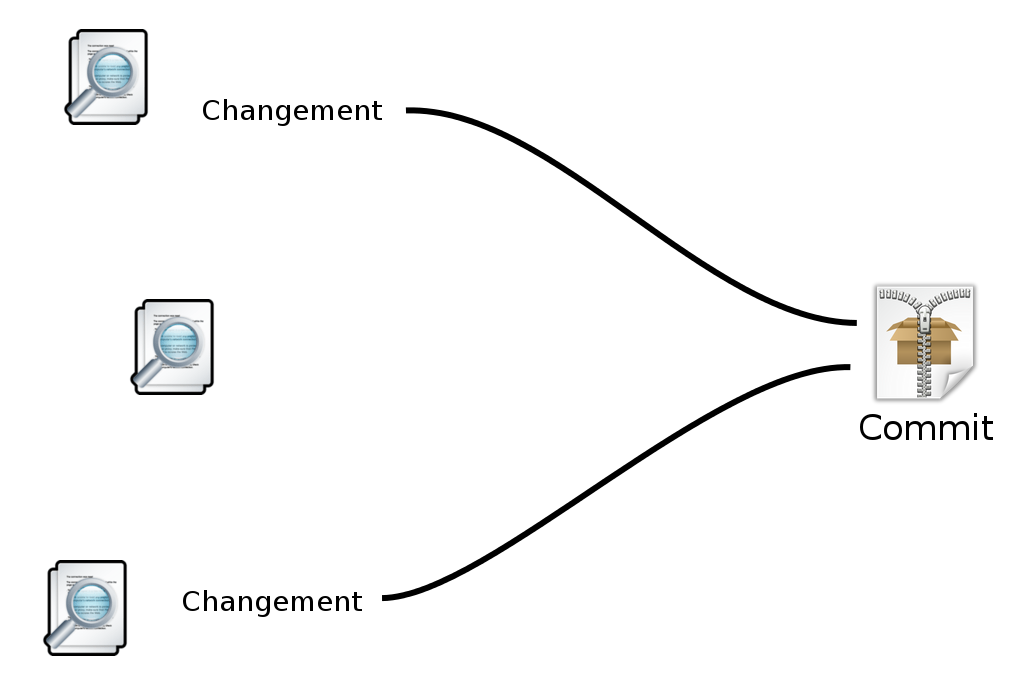
\includegraphics[scale=0.25]{commit.png}
\caption{Processus de création de commit}
\end{figure}

Ensuite chaque commit est envoyé vers le dépôt centrale, cette opération s'appelle la fusion. Chaque utilisateurs devra ensuite récupérer tout les commits envoyés et les fusionnés avec ça copie du dépôt. Si deux commits modifient la même partie d'un fichier, il y a ce que l'on appel un \textbf{conflit} et c'est à l'utilisateur de le résoudre en indiquant à Git qu'elle version garder.

Le répertoire \emph{.git} contient la liste de tout les commit, les configurations propres au dépôts, les branches, l'adresse du dépôt central. En gros, c'est ce qui permet à git de suivre correctement le projet, il convient donc de ne pas y toucher.

%%TODO : Ajouter la partie sur l'installation

\section{Premier dép\^ot}

Pour apprendre, rien de mieux que d'essayer par sois-même, nous allons donc ici faire un dépôt d'expérimentation, pas à pas, et nous détaillerons chaque commande utilisées.

\subsection{Création du dép\^ot}

Nous souhaitons créer ici un dépôt qui contiendra le texte de votre rapport de stage. Pour cela il faut créer un dossier racine qui sera le répertoire du rapport.

\begin{verbatim}
mkdir rapport
cd rapport
\end{verbatim}

Une fois créer, on va transformer ce répertoire en dépôt Git. Pour cela on utilise la commande :

\begin{verbatim}
git init

// Résultat
Initialized empty Git repository in /home/antoine/rapport/.git/
\end{verbatim}

La commande \emph{git init} va créer le répertoire \emph{.git} et va l'initialiser pour gérer un nouveau dépôt.

\subsection{Le premier commit}

Maintenant que le dépôt est créer, il faut le remplir. Pour cela on créer les fichier normalement comme s'il s'agissait d'un dossier normal. Ensuite on fait ses premières modifications puis viens l'heure du commit. Créez un fichier \emph{rapport.txt} puis ajoutez-y 2-3 lignes.

Voyons maintenant ce que Git à détecter :

\begin{verbatim}
git status

//Résultat
# On branch master
#
# Initial commit
#
# Untracked files:
#   (use "git add <file>..." to include in what will be committed)
#
#	rapport.txt
nothing added to commit but untracked files present (use "git add" to track)
\end{verbatim}

Notre fichier rapport.txt a bien été créer, cependant Git ne sait pas quoi faire avec. Il faut lui indiquer que notre rapport doit être ajouté pour commit (traqué). La commande \textbf{git add} permet de faire ça.

\begin{verbatim}
git add rapport.txt

git status

//Résultat
# On branch master
#
# Initial commit
#
# Changes to be committed:
#   (use "git rm --cached <file>..." to unstage)
#
#	new file:   rapport.txt
#
\end{verbatim}

Le fichier rapport.txt est donc en attente pour être committé. Il n'y a donc plus qu'a créer le commit

\begin{verbatim}
git commit
\end{verbatim}

Un éditeur de texte en mode console s'ouvrira alors (vi, vim ou nano). Entrez alors une description du commit, enregistrez et c'est terminé.

\paragraph{Note :}Dans vos nom de commit, entrez des petite phrases simples et évitez les fioritures. Utilisez des verbes conjugués au présent. Exemple : \textit{Corrige l'envoie des weekmails}.

\subsection{Modifier le dep\^ot}

Lorsque l'on travaille avec Git, il y a trois grandes étapes à respecter qui forme un cycle : 
\begin{itemize}
\item Modifier le code source
\item Tester les modifications
\item Valider les modifications en effectuant un commit
\end{itemize}

Modifier le code source signifier modifier n'importe quel fichier faisant partie du dép\^ot. Ca peut aussi bien être qu'une ligne changé dans un fichier que 25 dans un fichier A et 510 dans un fichier B. Ce qu'il faut se demander c'est : Est-ce que les modifications que j'effectue me permettent de corriger le bug ou d'ajouter la fonctionnalité dont j'ai besoin.

Faites quelques modifications sur votre rapport.

Ensuite utilisez la commande la commande \textit{git diff}. Cette commande permet d'afficher toutes les modifications apportées au project depuis le dernier commit. Voici un exemple de sortit possible

\begin{verbatim}
diff --git a/src/Symfony/Components/Yaml/Yaml.php b/src/Symfony/Components/Yaml/
index fa0b806..77f9902 100644
--- a/src/Symfony/Components/Yaml/Yaml.php
+++ b/src/Symfony/Components/Yaml/Yaml.php
@@ -19,7 +19,7 @@ namespace Symfony\Components\Yaml;
  */
 class Yaml
 {
-    static protected $spec = ’1.2’;
+    static protected $spec = ’1.3’;

     /**
      * Sets the YAML specification version to use.
@@ -33,6 +33,8 @@ class Yaml
         if (!in_array($version, array(’1.1’, ’1.2’))) {
             throw new \InvalidArgumentException(sprintf(’Version %s of the YAML
         }
+
+        $mtsource = $version;

         self::$spec = $version;
     }
\end{verbatim}

Les lignes commençant par + indiquent un ajout. Les lignes commençant par - indiquent un suppression.

Une fois que vous êtes satisfait de vos modifications \textbf{et que vous êtes sûr qu'elles fonctionnent}, il faut les committé pour les valider de façon définitive.

Il y a trois façons de faire

\begin{itemize}
\item \emph{git add fichier1 fichier2 etc} puis \emph{git commit}, comme vu précédemment 
\item \emph{git commit fichier1 fichier 2 etc}, c'est équivalent à la commande précédente en plus condensé
\item \emph{git commit -a}, commit tous les fichiers modifiés
\end{itemize}

Ensuite, on retrouve la procédure vue précédemment, le message de commit à saisir, etc.

\subsection{Commandes utiles}

Voici une liste de quelques commandes utiles qui vous sauveront surement plus d'une fois la vie.

\subsubsection{Modifier un commit}

En cas de problème suite à un commit il est toujours possible de le modifier, voire de l'annuler.

\paragraph{Modifier le message de commit :}Pour modifier le message du dernier commit, on peut utiliser la commande:
\begin{verbatim}
git commit --amend
\end{verbatim}
L'éditeur de texte s'ouvrira permettant de modifier le message de commit.

\paragraph{Annuler un commit}Pour annuler un commit avec la méthode douce, c'est-à-dire sans perdre les modifications effectués, on utilise la commande

\begin{verbatim}
git reset HEAD^
\end{verbatim}
Ce qui fera revenir le dépot à l'avant dernier commit sans perdre aucune modifications.

HEAD désigne le dernier commit, HEAD\^{} l'avant dernier, HEAD-2 l'avant avant dernier, etc.

La méthode forte annule le commit + les changements effectués. (\textbf{Cette commande est irréversible !})

\begin{verbatim}
git reset --hard HEAD^
\end{verbatim}

\paragraph{Astuce : Annuler les changement non commités} En utilisant la commande précédente, il est possible d'annuler les changements non committés

\begin{verbatim}
git reset --hard HEAD
\end{verbatim}

\paragraph{Annuler les changements apportés à un fichier non committé} Pour faire ça, la commande est différente :

\begin{verbatim}
git checkout fichier
\end{verbatim}

\subsubsection{Contrôler qui à fait quoi}

Ces commandes ne trouveront par forcement leur utilité dans le cadre d'un projet personnel, mais elles deviennent vite indispensable quand le projet englobe plusieurs personnes.

\paragraph{Qui a modifier cette ligne ?} Pour répondre à cette question, il y a la commande \emph{git blame}

\begin{verbatim}
git blame poly_git.tex

Résultat

aa6631b0 (Eryldor           2013-03-30 12:50:33 +0100   1) \documentclass[a4paper]{article}
aa6631b0 (Eryldor           2013-03-30 12:50:33 +0100   2) 
aa6631b0 (Eryldor           2013-03-30 12:50:33 +0100   3) \usepackage[utf8]{inputenc}
aa6631b0 (Eryldor           2013-03-30 12:50:33 +0100   4) \usepackage[T1]{fontenc}
aa6631b0 (Eryldor           2013-03-30 12:50:33 +0100   5) \usepackage[francais]{babel}
aa6631b0 (Eryldor           2013-03-30 12:50:33 +0100   6) \usepackage[top=2cm,bottom=2cm,left=3cm,right=2cm]{geometry}
aa6631b0 (Eryldor           2013-03-30 12:50:33 +0100   7) \usepackage{setspace}
60814e0e (Eryldor           2013-03-30 18:46:52 +0100   8) \usepackage{graphicx}
aa6631b0 (Eryldor           2013-03-30 12:50:33 +0100   9) 
aa6631b0 (Eryldor           2013-03-30 12:50:33 +0100  10) \title{Introduction à Git et à GitHub}
aa6631b0 (Eryldor           2013-03-30 12:50:33 +0100  11) \author{Antoine \bsc{Wacheux}}
aa6631b0 (Eryldor           2013-03-30 12:50:33 +0100  12) \date{30 mars 2013}
aa6631b0 (Eryldor           2013-03-30 12:50:33 +0100  13) 
aa6631b0 (Eryldor           2013-03-30 12:50:33 +0100  14) \onehalfspace
aa6631b0 (Eryldor           2013-03-30 12:50:33 +0100  15) 
aa6631b0 (Eryldor           2013-03-30 12:50:33 +0100  16) \begin{document}
aa6631b0 (Eryldor           2013-03-30 12:50:33 +0100  17) 
aa6631b0 (Eryldor           2013-03-30 12:50:33 +0100  18) \maketitle
aa6631b0 (Eryldor           2013-03-30 12:50:33 +0100  19) 
...
\end{verbatim}

Vous obtenez le hash du dernier commit (aa6631b0), l'auteur (Eryldor), la date (2013-03-30 12:50:33) et la ligne modifiée.

\paragraph{Quelles sont les dernier commits ?}

La aussi, une commande permet de retracer l'historique des commits : \emph{git log}

\begin{verbatim}
git log

Résultat

commit 0671bc8e48d0c2369cb04d504519e7380354f7e5
Author: Eryldor <eryldor.dev@gmail.com>
Date:   Sun Apr 28 14:34:51 2013 +0200

    Ajoute la partie sur la création de commit

commit 60814e0ee585d286c47282d902d462ff023a1355
Author: Eryldor <eryldor.dev@gmail.com>
Date:   Sat Mar 30 18:46:52 2013 +0100

    Ajoute la partie sur le fonctionnement global de git

commit 63efd91bf9b3b35bcf5ea0f823548d5ef5706191
Author: Eryldor <eryldor.dev@gmail.com>
Date:   Sat Mar 30 13:26:13 2013 +0100

    Section historique

commit aa6631b021d8699a6bf56a84d12cf1346ca1e2f1
Author: Eryldor <eryldor.dev@gmail.com>
Date:   Sat Mar 30 12:50:33 2013 +0100

    Ajoute le fichier LaTeX du poly

commit 004b61fc9901b58f3786ddc90c95d8f992d49b44
Author: Shiroy <wacant@free.fr>
Date:   Sat Mar 30 03:43:31 2013 -0700

    Initial commit
\end{verbatim}

Là aussi vous obtenez, la date, l'auteur, le hash avec en plus le message de commit.

\part{Travaillez à plusieurs, utilisez GitHub !}

\section{Présentation}

GitHub est un service web d'hébergement de source et de gestion de développement logiciel se basant sur Git. Ce site propose des comptes gratuits pour l'hébergement de logiciel libre et des comptes payant pour des dépôts privés\footnote{On peut également héberger des dépots privés gratuitement en utilisant un autre site web appelé Bitbucket}
GitHub propose en plus de l'hébergement plusieurs services : 
\begin{itemize}
\item Un suivi complet des dépôts par le site
\item Un bugtracker
\item Un système de wiki
\item Un système similaire à pastebin, nommé Gist
\end{itemize}

Parmi les projets hébergé su ce site, on peut cité:
\begin{itemize}
\item Tous les projets informatiques de FabLabUTC\footnote{https://github.com/FabLabUTC}
\item PayUTC \footnote{https://github.com/payutc}
\item Le portail des assos de l'UTC \footnote{https://github.com/simde-utc/portail}
\item Beaucoup d'autres projets libres.
\end{itemize}

\begin{figure}
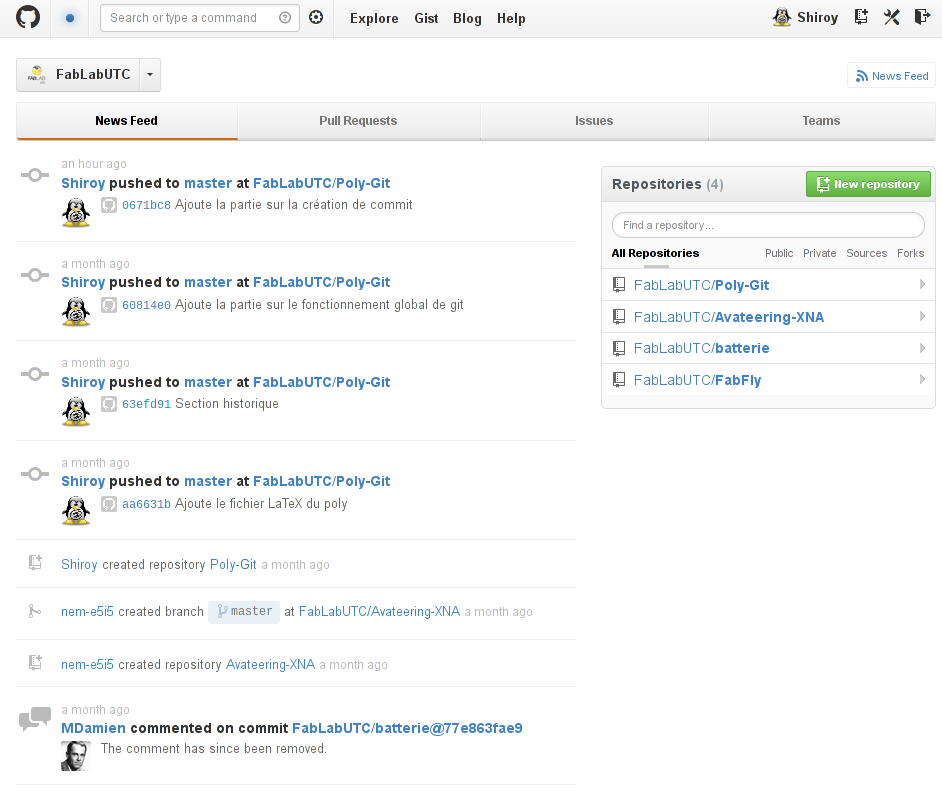
\includegraphics[scale=0.6]{accueil_github.png}
\label{Page d'accueil de GitHub}
\caption{Page d'accueil de GitHub}
\end{figure}

A présent, nous allons héberger notre rapport sur GitHub. Si vous n'avez pas de compte, créez vous en un, sinon connectez vous.

\section{Création d'un dépôt GitHub}

La création du dépôt se fait de manière assez intuitive, il y a un bouton \og New repository \fg sur lequel il suffit de cliquer.

\paragraph{Note : }Si vous avez un dépôt à mettre en ligne, créer un dépôt vide sans l'initialiser. Sinon vous pouvez cocher la case \og Initialize this repository with a README  \fg, ce qui créera un dépôt pré-fait avec un README et un .gitignore.

\begin{figure}
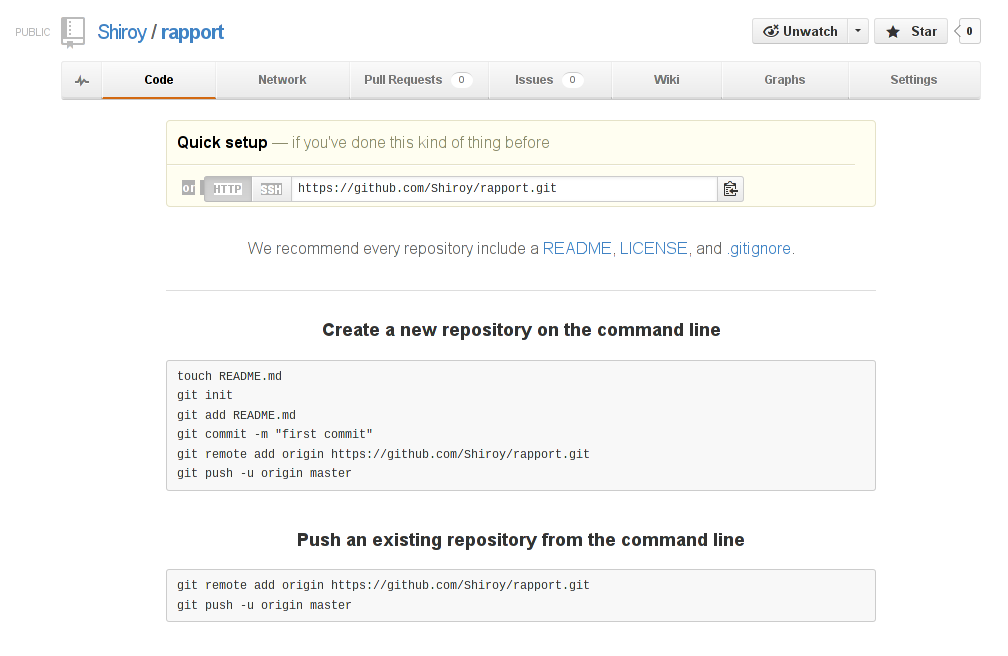
\includegraphics[scale=0.6]{creation_depot.png}
\caption{Création du dép\^ot rapport}
\end{figure}

Une fois créer, vous obtenez un écran ressemblant à la figure ci-dessous. En haut dans la barre du cadre \og Quick setup \fg se trouve l'adresse du dépôt qui va permettre à Git de s'y connecter pour faire la mise en ligne.

Maintenant, il faut indiquer à Git cette fameuse adresse. Il faut ajouter un remote.

\paragraph{Les remotes :}Un remote représente un ordinateur distant hébergeant le même dépôt que le votre. C'est ce système qui permet de complètement décentraliser Git. Cependant, on s'arrange en général pour tout centraliser sur un seul serveur car c'est beaucoup plus simple à gérer.

\paragraph{Ajout du remote GitHub} L'ajout se fait grâce à la commande :

\begin{verbatim}
git remote add <nom_remote> <url_remote>
\end{verbatim}

Le paramètre \emph{nom\_remote} indique un nom en local que vous utiliser pour identifier le remote dans votre liste. Par convention on  appelle le remote du serveur distant \textit{origin}. Ce qui nous donne donc.

\begin{verbatim}
git remote add origin <url_indiquée_par_GitHub>
\end{verbatim}

La dernière étape est de pousser les modifications sur le dépôt. En gros de les uploader. Pareil la commande est encore très simple.

\begin{verbatim}
git push -u origin master
\end{verbatim}

Vous reconnaissez ici origin, le nom de notre remote. Master désigne la branche à pousser (nous n'aborderons pas le concept de branche faute de temps). L'option -u permet de lier la branche master d'origin à la branche master locale, ainsi toutes modifications faites sur le serveur se répercutera automatiquement sur le dépôt local (ce qui parfois n'est pas forcement une bonne chose :) )

La commande qui fait l'inverse, c'est-à-dire qui récupère les données depuis le serveur est
\begin{verbatim}
git pull
\end{verbatim}

Ainsi en vous échangeant les adresse des dépôts (et en donnant les bon accès) vous pouvez travaillez à plusieurs sur un même projet sans prise de tête. Git se chargera de tout fusionné correctement et en cas de problème (conflit il vous demandera quoi faire).

\end{document}